\chapter{Tensor diagrams, invariant theory and quantum graph grammars}
\label{ch:tensor-grammars}
\reviewstatus{The finite-dimensional identities in this chapter are proved below. The accompanying executable laboratory checks concrete instances. The new Lean module formalizes a precisely stated sequential linear-map fragment and its contextual rewrite soundness; it is not a formalization of every tensor category, every graph grammar, or cosmology.}

\section{A diagram must have a type and an interpretation}

The common language needed for this project is more exact than a resemblance between pictures. A dessin is an embedded bipartite graph with a cyclic order at its vertices. A cell complex has boundary maps. A tensor network has labelled vector spaces and contracted indices. A circuit has an ordered causal composition and a measurement rule. A grammar has productions and an acceptance convention. One underlying graph may carry several of these structures, but the additional data have to be supplied. A surface embedding alone does not specify a Hamiltonian, a grammar, a quantum state, or a physical communication channel.

We work initially over $\C$ with finite-dimensional Hilbert spaces. Fix an orthonormal basis $e_i$ of each space $H$, and let $H^*$ denote its linear dual. A boundary type is a finite ordered tensor word in such spaces and their duals. The empty word denotes $\C$. A box $A:H\to K$ has components $A^j{}_i$; a wire joins an output of one box to an input of the same type of another. Repeated matching indices are summed over their full stated ranges. In particular,
\[
 (BA)^k{}_i=\sum_j B^k{}_j A^j{}_i,
 \qquad
 (A\otimes C)^{j\ell}{}_{ik}=A^j{}_i C^\ell{}_k.
\]
The drawing convention in this chapter places inputs on the left and outputs on the right, with the order of tensor factors specified at every boundary. Reflection accompanied by complex conjugation denotes the adjoint; reflection alone is not the adjoint of a complex matrix.

This is a concrete finite-dimensional instance of the graphical language surveyed by Selinger, while the invariant-tensor calculations below follow the purpose of Cvitanovi\'c's birdtracks: lines carry representation indices and vertices carry specified invariant tensors \cite{TGselinger,TGbirdtracks}. We use component proofs for the identities actually needed, without importing an unrestricted diagrammatic coherence assertion.

\begin{proposition}[Elementary diagram semantics]
For composable linear maps the following identities hold:
\begin{align*}
 (B\otimes D)(A\otimes C)&=BA\otimes DC,\\
 (BA)^\dagger&=A^\dagger B^\dagger,\\
 (A\otimes C)^\dagger&=A^\dagger\otimes C^\dagger.
\end{align*}
The swap $S_{H,K}:H\otimes K\to K\otimes H$, defined by
$S(x\otimes y)=y\otimes x$, is unitary, has inverse $S_{K,H}$, and satisfies
$S_{H',K'}(A\otimes C)=(C\otimes A)S_{H,K}$.
\end{proposition}
\begin{proof}
The $(j,\ell;i,k)$ component of the first left-hand side is
$\sum_{a,b}B^j{}_aD^\ell{}_bA^a{}_iC^b{}_k$.
The finite sum factors into $(BA)^j{}_i(DC)^\ell{}_k$.
For the adjoint, $(A^\dagger)^i{}_j=\overline{A^j{}_i}$; taking the conjugate of the finite matrix-product sum reverses its order. The tensor assertion follows from conjugating the product of entries. The swap permutes an orthonormal tensor basis, hence is unitary. Applying the remaining identities to $x\otimes y$, a spanning set, proves them.
\end{proof}

Evaluation and coevaluation are the maps
\[
 \epsilon_H:H^*\otimes H\to\C,\quad f\otimes x\mapsto f(x),
 \qquad
 \eta_H(1)=\sum_i e_i\otimes e^i\in H\otimes H^*.
\]
Although displayed in coordinates, $\eta_H$ is basis independent: under $e'_i=\sum_jM^j{}_ie_j$, the dual basis uses $M^{-1}$ and their coefficients contract to a Kronecker delta. These maps are the cup and cap of the diagram language. They are algebraic maps, not automatically normalized state preparation and measurement operations.

\begin{proposition}[Snake identity and the closed loop]
The composite
$(\operatorname{id}_H\otimes\epsilon_H)(\eta_H\otimes\operatorname{id}_H)$
is $\operatorname{id}_H$. Closing the output of $A\in\End(H)$ against its input gives $\Tr A$. An empty closed $H$-wire evaluates to $\dim H$.
\end{proposition}
\begin{proof}
For $x=\sum_jx_je_j$, the first composite is
$\sum_i e_i e^i(x)=x$. The closed diagram for $A$ is
$\sum_i e^i(Ae_i)=\sum_iA^i{}_i$. Taking $A$ to be the identity gives the dimension. The other snake identity follows by evaluating a dual basis vector in the same way.
\end{proof}

For $\dim H=d>0$, the cup has squared norm $d$. A physical maximally entangled state uses $d^{-1/2}\eta_H$ after a chosen identification of the dual factor with a laboratory register. Using normalized cups at both ends changes a snake contraction by $d^{-1}$. Ignoring that scalar would change success probabilities. This small distinction is essential when a birdtrack identity becomes an actual quantum circuit.

\section{Wedge powers, Young symmetry and determinants as diagrams}

The symmetric group acts unitarily on $H^{\otimes r}$ by
\[
 P_\sigma(x_1\otimes\cdots\otimes x_r)
 =x_{\sigma^{-1}(1)}\otimes\cdots\otimes x_{\sigma^{-1}(r)}.
\]
Crossings represent these permutations. In characteristic zero define
\[
 A_r=\frac1{r!}\sum_{\sigma\in S_r}\operatorname{sgn}(\sigma)P_\sigma,
 \qquad S_r^{\rm sym}=\frac1{r!}\sum_{\sigma\in S_r}P_\sigma.
\]
These are alternating and symmetric projectors. Over an integral ring the denominators cannot simply be inserted: the Schur constructions and straightening relations of the earlier chapters are precisely what permits a formulation before inverting factorials.

\begin{proposition}[Alternating projector and its rank]
$A_r^2=A_r=A_r^\dagger$. Its image has an orthogonal basis indexed by strictly increasing $r$-tuples in $\{1,\ldots,d\}$, so
$\Tr A_r=\binom dr$, interpreted as zero if $r>d$. For $r=2$,
\[
 A_2=\tfrac12(I-S),\qquad S_2^{\rm sym}=\tfrac12(I+S),
 \quad \Tr A_2=\tfrac12(d^2-d).
\]
\end{proposition}
\begin{proof}
In the double sum for $A_r^2$, for each $\tau$ there are $r!$ pairs $(\sigma,\rho)$ with $\sigma\rho=\tau$, and their sign product is $\operatorname{sgn}(\tau)$. This proves idempotence. Since $P_\sigma^\dagger=P_{\sigma^{-1}}$ and inversion preserves sign, it is self-adjoint. A tensor basis vector with repeated entries alternates to zero: exchanging the repeated positions pairs equal terms with opposite signs. Otherwise its alternating image is a signed copy of the image associated to its sorted tuple. Distinct sorted tuples have disjoint tensor-basis supports, so these nonzero images are orthogonal and span the image. Their number is $\binom dr$. Finally $S$ fixes exactly the $d$ diagonal tensor basis vectors in the trace, so $\Tr S=d$ and $\Tr I=d^2$.
\end{proof}

General Young diagrams use row symmetrization and column antisymmetrization in a specified order. Their product is generally not an orthogonal projector as written, and normalizing or orthogonalizing it is a separate operation. We do not replace the integral Schur module by that product in characteristics dividing its normalization. The standard monomial theory already developed supplies the required relations and bases; the diagram notation now makes the permutations and contractions visible. In particular, a shuffling relation is a linear identity among permutation diagrams, not a license to exchange arbitrary noncommuting circuit gates.

For a map $A:H\to K$, define $\bigwedge^r A$ on decomposables by
$x_1\wedge\cdots\wedge x_r\mapsto Ax_1\wedge\cdots\wedge Ax_r$.
Alternation makes this well-defined. In the increasing-tuple bases, its entries are the $r\times r$ minors of $A$.

\begin{proposition}[Exterior functoriality and Cauchy--Binet]
For $A:H\to K$ and $B:K\to L$,
\[
 \bigwedge^r(BA)=(\bigwedge^r B)(\bigwedge^r A).
\]
Equivalently, for increasing $r$-tuples $I,J$ of output and input indices,
\[
 \det(BA)_{I,J}=\sum_{|K|=r}\det B_{I,K}\det A_{K,J}.
\]
If $BA=0$ and $r>0$, the displayed composite is zero. For $r=0$ it is the identity of the ground field, so the last conclusion would be false.
\end{proposition}
\begin{proof}
Both maps in the first equation send a decomposable $r$-vector to
$BAx_1\wedge\cdots\wedge BAx_r$. Such vectors span. Expanding the intermediate image in its increasing-tuple basis yields exactly the finite minor sum. Alternatively, in the multilinear expansion of $BAx_1\wedge\cdots\wedge BAx_r$, repeated intermediate indices vanish and the $r!$ orderings of each distinct set assemble into a determinant. When $BA=0$ every factor is zero and $r>0$; the empty wedge in degree zero is $1$.
\end{proof}

The determinant is thus the action on the one-dimensional top exterior power. In coordinates it is an epsilon-tensor contraction. The Pl\"ucker relation for two vectors in a four-dimensional space expresses decomposability:
\[
 p_{12}p_{34}-p_{13}p_{24}+p_{14}p_{23}=0,
 \qquad p_{ij}=x_i y_j-x_j y_i.
\]
Each of the twelve expanded terms cancels with another after commuting scalar coefficients. This is the same exact relation checked by the existing algebra laboratory. Its graphical use preserves the typed external legs and coefficients. The minors, Schur modules, and invariant contractions thereby refer to the same algebraic constructions, rather than three unrelated kinds of pictures.

\section{A color contraction with every normalization fixed}

Let $N\ge2$ and choose traceless Hermitian matrices $T^a$, $1\le a\le N^2-1$, with $\Tr(T^aT^b)=\delta_{ab}/2$. They form a real basis of traceless Hermitian matrices and a complex basis of traceless matrices. An adjoint-index edge joins two generators; each generator also carries one incoming and one outgoing fundamental index.

\begin{proposition}[Fundamental completeness and Casimir]
\label{prop:fierz}
For $1\le i,j,k,l\le N$,
\[
 \sum_a (T^a)^i{}_j(T^a)^k{}_l
 =\frac12\left(\delta^i{}_l\delta^k{}_j
          -\frac1N\delta^i{}_j\delta^k{}_l\right),
 \qquad
 \sum_aT^aT^a=\frac{N^2-1}{2N}I.
\]
\end{proposition}
\begin{proof}
The matrices $I/\sqrt N$ and $\sqrt2 T^a$ form an orthonormal basis of $\End(\C^N)$ for $\langle A,B\rangle=\Tr(A^\dagger B)$. Expanding an arbitrary matrix $X$ in this basis gives
$X=\Tr(X)I/N+2\sum_aT^a\Tr(T^aX)$.
Compare the coefficient of the independent entry $X^l{}_k$ in its $(i,j)$ entry. This yields the first identity. Set $k=j$ and sum over $j$: the right-hand side becomes
$\frac12(N-1/N)\delta^i{}_l$.
\end{proof}

\begin{figure}[htbp]
\centering
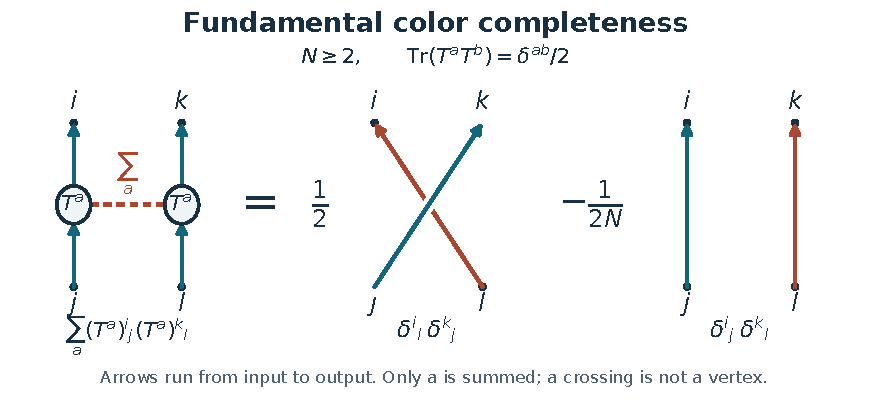
\includegraphics[width=\textwidth]{figures/second-pass-fierz.pdf}
\caption{The fundamental completeness relation with its four external indices and every coefficient. In this figure fundamental wires run vertically, from the explicitly labelled inputs to outputs. The dotted adjoint edge denotes summation over the normalized generators.}
\label{fig:second-pass-fierz}
\end{figure}

The first term on the right joins opposite fundamental legs; the second joins each pair without exchanging them. The factor $1/N$ and the factor $1/2$ are part of the theorem. A diagram that suppresses them is not the same invariant. This contraction is relevant to color indices in Yang--Mills calculations, but it evaluates a finite representation-theoretic factor. It supplies no continuum measure, renormalization estimate, or lower spectral bound. The earlier analytic obligations remain in force.

\section{Channels as positive tensors}

To discuss noisy circuits, learned measurements, and any proposed cross-aeon message, a linear amplitude map is insufficient. A density operator $\rho$ is positive semidefinite with trace one. A channel $\mathcal E:\End(H)\to\End(K)$ is completely positive and trace preserving. In the input-first convention its Choi tensor is
\[
 J_{\mathcal E}=\sum_{i,j}|i\rangle\langle j|\otimes
          \mathcal E(|i\rangle\langle j|).
\]
Here $|i\rangle\langle j|$ is a matrix unit; the outer input leg is conjugated when interpreted as a transformation rule under basis change. The convention is explicit so a transpose cannot be silently replaced by a dagger.

\begin{theorem}[Finite Choi--Kraus criterion]
\label{thm:choi-criterion}
Let $\mathcal E:\End(H)\to\End(K)$ be complex-linear. It is completely positive exactly when $J_{\mathcal E}\succeq0$. In that case there are matrices $K_\alpha:H\to K$ such that
\[
 \mathcal E(X)=\sum_\alpha K_\alpha X K_\alpha^\dagger.
\]
It is trace preserving exactly when
$\sum_\alpha K_\alpha^\dagger K_\alpha=I_H$, equivalently
$\Tr_KJ_{\mathcal E}=I_H$.
\end{theorem}
\begin{proof}
If $\mathcal E$ is completely positive, apply $\operatorname{id}_H\otimes\mathcal E$ to the positive operator $|\Omega\rangle\langle\Omega|$, where $\Omega=\sum_ie_i\otimes e_i$ in a basis-labelled copy of $H\otimes H$. Its image is $J_{\mathcal E}$.
Conversely diagonalize the positive matrix as $J=\sum_\alpha v_\alpha v_\alpha^\dagger$, incorporating square roots of eigenvalues into the vectors. Write
$v_\alpha=\sum_i e_i\otimes K_\alpha e_i$; this defines every matrix entry of $K_\alpha$ uniquely. The $(i,j)$ block of $J$ is then
$\sum_\alpha K_\alpha|i\rangle\langle j|K_\alpha^\dagger$.
Equality on matrix units proves the Kraus formula. Each map
$\operatorname{id}_m\otimes\mathcal E$ sends a positive $Y$ to
$\sum_\alpha(I_m\otimes K_\alpha)Y(I_m\otimes K_\alpha)^\dagger$, which is positive, proving complete positivity.
Finally cyclicity of the finite trace gives
$\Tr\mathcal E(X)=\Tr(X\sum_\alpha K_\alpha^\dagger K_\alpha)$.
The trace pairing is nondegenerate, so equality with $\Tr X$ for all matrix units is equivalent to the stated matrix identity. Taking the partial trace of the Choi formula gives the transpose of this sum; equality to $I$ is unchanged by transpose.
\end{proof}

The positive cone intersected with the affine partial-trace constraint gives a concrete feasible set for a learned channel. It differs from the affine variety $BA=0$: positivity is an inequality, not a polynomial equality over $\C$. With real and imaginary coordinates, the channel condition can be written as polynomial equalities together with nonnegative principal minors. This is a semialgebraic constraint. The geometry of complexes may constrain other blocks of a model, but it cannot replace the channel's positivity test.

An isometry or unitary circuit followed by a partial trace automatically produces a channel. A free matrix-valued neural output does not. One practical parameterization is to output a unitary dilation and trace an environment. Another is to parameterize Kraus operators and explicitly enforce their completeness relation. Renormalizing arbitrary operators without checking invertibility or the remaining constraints is not a proof of trace preservation.

\section{A precise grammar for the executable circuits}

We now separate three different questions. \emph{Generation} asks which finite graphs or circuit strings a grammar produces. \emph{Interpretation} maps each well-typed expression to a matrix or channel. \emph{Acceptance} asks what decision is made from a measurement or a classical computation on that interpretation. Their complexities can differ greatly.

For the finite laboratory let the wire type be $Q=\C^2$, with $1\le n\le6$. A gate record consists of a symbol from $\{H,X,Z,S,S^\dagger,T,T^\dagger,\mathrm{CX},\mathrm{SWAP}\}$ and a valid ordered list of distinct wire indices of the correct arity. A circuit is a sequence of such records; time runs from left to right and its matrix is the corresponding right-to-left product. Parameters such as $R_y(\theta)$ belong to a separate numerical experiment unless an angle alphabet or a computable encoding has been specified. Arbitrary real numbers are not a finite grammar alphabet.

A graph representation replaces each wire by a chain of directed edges and each gate by a typed vertex. Its input and output ports retain their order. In surface-constrained mode, allowed two-qubit gates must follow a supplied adjacency relation between data qubits on the cellulation. Relabelling vertices changes index names consistently, including the adjacency relation. A gate sequence is not a new dessin merely because it was rendered near a torus.

There are two useful kinds of production. A \emph{generative} production appends an allowed gate and changes the represented unitary. An \emph{equational} production replaces a subdiagram by an equal map and preserves the represented unitary. The laboratory's cancellation rule removes adjacent $U,U^\dagger$ on the same ordered wires. It also exposes commuting disjoint gates as an independently checked identity. No rule treats an approximate learned equality as exact.

\begin{theorem}[Typed rewrite soundness]
\label{thm:typed-rewrite-soundness}
Interpret a well-typed expression using composition, tensor product, and the specified generator maps. Suppose every equational rule $L\rightsquigarrow R$ has the same input and output type and $\llbracket L\rrbracket=\llbracket R\rrbracket$. Replacing any subexpression by such a rule preserves the full interpretation. For unitary circuit interpretations, every finite sequence of these replacements preserves every output measurement probability on every input density operator.
\end{theorem}
\begin{proof}
An expression with one hole is built from the hole by successively composing on either side with a fixed map or tensoring on either side with a fixed map. Equality is preserved by each operation, using bilinearity or simply substitution. Induction on this construction proves equality in every context. Induction on the number of rewrites proves equality after a finite derivation. Equal circuit matrices $U,V$ give equal operators $U\rho U^\dagger=V\rho V^\dagger$, and hence equal numbers $\Tr(MU\rho U^\dagger)$ for every measurement effect $0\preceq M\preceq I$.
\end{proof}

\begin{figure}[htbp]
\centering
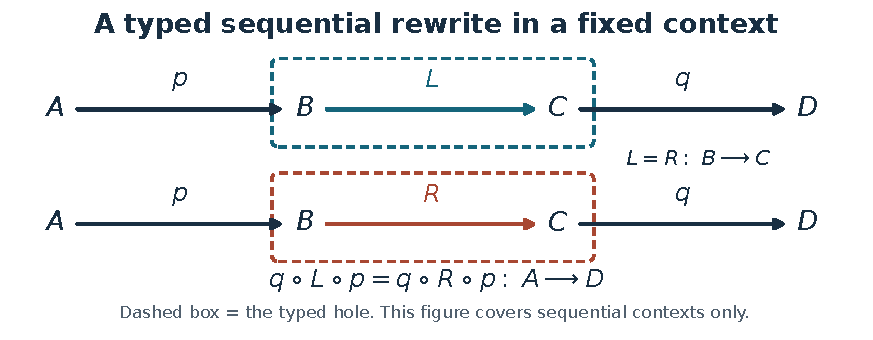
\includegraphics[width=\textwidth]{figures/second-pass-typed-context.pdf}
\caption{A typed sequential context. An equality of maps with the same domain and codomain can be substituted between fixed maps. The formal module checks this sequential syntax and finite derivations; tensor extensions are proved in the text.}
\label{fig:second-pass-context}
\end{figure}

The Lean file verifies the sequential linear-map part of this argument with a typed syntax and one-hole contexts. Tensor-context cases and density-operator consequences are proved in the text. This is an exact scope statement: checking the sequential theorem does not certify a parser, graphical embedding, tensor coherence theorem, or browser floating-point arithmetic.

\begin{proposition}[Termination and accumulated approximation error]
Repeated adjacent inverse cancellation terminates. If $U_j,V_j$ are unitary operators on the same Hilbert space and $\|U_j-V_j\|\le\epsilon_j$, then
\[
 \|U_m\cdots U_1-V_m\cdots V_1\|\le\sum_{j=1}^m\epsilon_j.
\]
For a unit input vector and a measurement effect of norm at most one, the resulting probability difference is at most $2\sum_j\epsilon_j$.
\end{proposition}
\begin{proof}
Every cancellation reduces the nonnegative integer number of gates by two. For the norm bound, insert products whose first $j$ factors have been replaced and telescope. Each difference is a left unitary product times $U_j-V_j$ times a right unitary product, so its norm is at most $\epsilon_j$. For output vectors $u,v$,
$\langle u,Mu\rangle-\langle v,Mv\rangle
=\langle u-v,Mu\rangle+\langle v,M(u-v)\rangle$.
Cauchy--Schwarz and $\|u\|=\|v\|=1$ give the stated bound.
\end{proof}

Termination is not completeness. A circuit with no adjacent inverse pair may still equal the identity; for example $(HZ)^8$ does. The chosen local simplifier is allowed to miss an equality. Its guarantee is that every equality it does apply is valid. A learned policy can rank applicable valid rewrites without changing this guarantee. If it is also allowed to propose new identities, a separate certificate or numerical-error bound must be checked before acceptance.

\section{How the grammar preserves a complex}

The varieties-of-complexes constraint can be carried through a learned representation without pretending that any graph mutation preserves it. Let
$C_2\xrightarrow{d_2}C_1\xrightarrow{d_1}C_0$ satisfy $d_1d_2=0$.

\begin{proposition}[Transport of a complex and its metric]
\label{thm:unitary-chain-transport}
Let $F_i:C_i\to C'_i$ be invertible linear maps and put
$d'_i=F_{i-1}d_iF_i^{-1}$. Then $d'_1d'_2=0$, and $F_1$ induces an isomorphism
$\ker d_1/\im d_2\cong\ker d'_1/\im d'_2$.
If the spaces carry Hilbert metrics and all $F_i$ are unitary, the middle Laplacians satisfy
\[
 d_1'^\dagger d'_1+d'_2d_2'^\dagger
 =F_1(d_1^\dagger d_1+d_2d_2^\dagger)F_1^{-1}.
\]
\end{proposition}
\begin{proof}
The middle inverse cancels in
$d'_1d'_2=F_0d_1F_1^{-1}F_1d_2F_2^{-1}=0$.
The same identities show $F_1(\ker d_1)=\ker d'_1$ and
$F_1(\im d_2)=\im d'_2$, giving a well-defined invertible quotient map. When $F_i^{-1}=F_i^\dagger$, taking adjoints of the transported differentials and cancelling the adjacent unitary factors gives the displayed conjugacy term by term.
\end{proof}

Invertibility alone gives homology invariance; it does not give this spectral equality for fixed metrics. This is the same algebra-versus-metric distinction encountered in lattice cryptography. A learned basis change should therefore specify whether it preserves the inner product, changes the metric along with the basis, or deliberately changes the spectrum.

\begin{proposition}[A controlled enlargement]
Adjoin the two-term complex $0\to W\xrightarrow{I}W\to0$ in any adjacent degrees, with zero couplings to the original complex. The direct-sum complex has the same homology as the original. With orthogonal direct-sum metrics its Laplacian gains an eigenvalue equal to one with multiplicity $\dim W$ in each of those two degrees.
\end{proposition}
\begin{proof}
The added identity has zero kernel and full image, so its two homology groups vanish. Kernels and images of a block-diagonal differential decompose into direct sums, yielding the homology assertion. On each new $W$ summand precisely one of $d^\dagger d$ and $dd^\dagger$ is $I$ and the other is zero. Thus its Laplacian block is $I$.
\end{proof}

This is an elementary grammar rule for increasing representation size with a proof of homological preservation. It is not automatically a geometric subdivision of a given surface; constructing the required cellular chain equivalence is an additional task. It also shows why preserving homology does not preserve a numerical gap unchanged: when $W\ne0$, a former gap greater than one in an affected degree becomes one after this enlargement.

\section{Expressivity: four different classifications}

The Chomsky hierarchy classifies languages of finite strings over a finite alphabet. A graph language enters that hierarchy only after a serialization and acceptance relation have been specified. The label ``context-free graph grammar'' does not assert that every natural string yield is a context-free language. Hyperedge replacement has its own gluing semantics and expressive distinctions \cite{TGhrg}.

\begin{proposition}[Bounded interfaces give bounded treewidth]
Consider a finite hyperedge replacement grammar. A production replaces one nonterminal hyperedge by a fixed finite graph with an ordered external interface; the only identifications are the prescribed attachment vertices, distinct external vertices remain distinct, and new internal vertices are fresh. Suppose every right-hand side and the initial graph has at most $b$ vertices. For every finite complete derivation, the primal graph of its terminal result has a tree decomposition of width at most $b-1$.
\end{proposition}
\begin{proof}
Use the derivation tree, with a root for the initial graph and one node for each replacement. At each node place in a bag the images in the final graph of all vertices in its right-hand side, including its external vertices; at the root use the initial vertices. Each bag has at most $b$ vertices. Every final vertex was either initial or introduced by a production and lies in its creating bag. Every pair of vertices made adjacent by a terminal hyperedge occurs together in the bag in which that hyperedge was introduced. Finally, a vertex can enter a descendant production only through the attachment interface of a hyperedge already containing it. Along the unique ancestry path from its creation to any later occurrence, it therefore remains in every intervening bag. Its bags form a connected subtree. These are exactly the covering, edge, and connectedness conditions for a tree decomposition.
\end{proof}

The bound applies to a fixed grammar with fixed finite production templates. It does not cover an arbitrary new gate layer supplied as an unbounded template, unbounded interfaces, or later identifications of distant vertices. In particular, a fixed bound cannot generate all increasingly large square grids: their treewidth is unbounded. This limits what a narrow-interface grammar can express on larger and higher-genus surface-code families.

\begin{proposition}[Context-free graph generation can have a non-context-free string yield]
A fixed-interface graph grammar with distinct attachment vertices can generate path graphs with edge labels
$a^n\#b^n\#c^n$, $n\ge1$. Their left-to-right string language, and its yield after erasing the two separators, are not context free.
\end{proposition}
\begin{proof}
Use a nonterminal with six distinct external vertices, the endpoints of three ordered paths. Its base production makes three one-edge paths labelled $a,b,c$. Its recursive production extends the first path by one $a$, the second by one $b$, and the third by one $c$, passing their new endpoints as the interface of one recursive occurrence. An initial production adds one separator-labelled edge from the end of the first path to the start of the second and another from the end of the second to the start of the third, producing one path without identifying any attachment vertices. Equivalently its three-component yield obeys
$(x,y,z)\mapsto(ax,by,cz)$ from $(a,b,c)$, followed by separator insertion. Induction gives the stated graph language and, after erasure, $\{a^nb^nc^n:n\ge1\}$.
If the latter language were context free, let $p$ be a pumping length and consider $a^pb^pc^p$. In any pumping decomposition with the central three-piece block of length at most $p$, that block meets at most two adjacent constant-letter blocks. Pumping the two designated pieces changes at least one count, leaves at least one of the three counts unchanged, and either destroys the letter order or makes the counts unequal. The pumped string is outside the language, contradicting the pumping property. Finally, erasing a terminal in the productions of a context-free grammar yields a context-free grammar for the erased language, allowing empty productions. Thus the separator-containing language cannot have been context free either.
\end{proof}

The example's final graphs are paths, so their treewidth is only one. Graph width, language yield complexity, and quantum simulation complexity are different quantities. The separator-erasing homomorphism is specified explicitly rather than hidden in an informal reading of the graph.

\begin{proposition}[Unrestricted effective graph rewriting can express Type-0 recognition]
Allow finite labelled graphs, local finite rewrite rules, unbounded graph growth, and acceptance when a distinguished accepting state is reached. This model can simulate every Turing machine. Its recognized input-string languages are exactly the recursively enumerable languages.
\end{proposition}
\begin{proof}
Represent a machine tape by a directed path of cells with symbol labels and a distinguished cell carrying the machine state. A transition changing symbol $a$ to $b$ and moving right is a local rewrite of the current head cell and its right neighbour: replace $a$ by $b$ and move the state marker to that neighbour. A second rule handles the end of the represented tape by creating a fresh blank cell. Left moves have analogous rules, with a fixed left-end marker for a one-sided tape. Since state and tape alphabets and the transition table are finite, there are finitely many rules. Induction on machine steps proves exact correspondence between configurations and reachable labelled paths. An accepting state is reached exactly when the machine accepts. Conversely, finite labelled graphs and finite rule matches have effective finite encodings. Breadth-first enumeration of finite derivations semi-decides whether an accepting graph is reachable. This gives the reverse inclusion.
\end{proof}

No general terminating algorithm decides all acceptance questions for that unrestricted model: such an algorithm would decide Turing-machine acceptance, contradicting diagonalization. Adding quantum amplitudes does not justify omitting computability assumptions on coefficients or providing a finite simulator with unbounded resources.

\begin{center}\small
\begin{tabular}{p{.25\linewidth}p{.32\linewidth}p{.34\linewidth}}
\toprule
Model & Precisely classified object & Consequence\\\midrule
Bounded browser laboratory & Finite circuits on at most six wires and a bounded gate count & A finite set; every serialization language is regular.\\
Fixed-width unbounded instruction strings & All well-typed instructions from a finite gate alphabet & Syntactic validity is regular; semantic equality is a different problem.\\
Finite-interface replacement grammar & Graphs glued through specified ports & A bounded-width graph class under the proposition's assumptions; string yields need not be context free.\\
Unrestricted effective rewriting & Existence of a finite accepting derivation & Type-0 recognition; general termination is undecidable.\\
Uniform polynomial quantum circuits & Bounded-error measurement decisions as input length grows & BQP, a computational complexity class, not an extra level of the Chomsky hierarchy.\\\bottomrule
\end{tabular}
\end{center}

For the last row, ``uniform'' means that a classical algorithm produces the size-$n$ circuit in polynomial time, using a fixed finite gate set with effectively computable entries. Bounded error means acceptance probability at least $2/3$ on yes instances and at most $1/3$ on no instances. Noncomputable real parameters would hide an oracle in the model. A fixed six-qubit browser demonstration is a finite numerical example, not evidence that an asymptotic BQP-hard problem has been solved efficiently.

\section{When the tensor grammar is also efficiently classical}

\begin{proposition}[Dynamic contraction along a derivation tree]
Suppose every tensor index has dimension at most $D$, each production has at most $q$ distinct local index variables including its external interface, and there are $m$ production instances. If child tensors are contracted and summarized at their prescribed interfaces, the final tensor can be computed with at most $O(mD^q)$ scalar operations, up to a fixed factor depending on the grammar. The bound assumes that the required final interface also fits within $q$.
\end{proposition}
\begin{proof}
Process the finite derivation tree from its leaves upward. At a production, the already computed child tensors and the finitely many local generator tensors have entries indexed by the at most $q$ local variables. Enumerate all their assignments, multiply the relevant entries, and add to the corresponding external-interface entry. There are at most $D^q$ assignments, and a fixed grammar bounds the number of factors per assignment. This computes exactly the contracted subdiagram by associativity and distributivity of finite sums. Summing the work over $m$ nodes proves the estimate.
\end{proof}

This explains an important tradeoff for quantum learning on diagrams. A bounded-interface family may be interpretable, trainable, and classically tractable for the same structural reason. It should be chosen for those benefits when appropriate; its tractability is not evidence of a quantum speedup. Conversely, allowing wide entangling interfaces can remove this contraction bound and make state-vector simulation exponential in the qubit count. The earlier GPU results distinguish dense amplitudes from stabilizer frames precisely for this reason.

The graph's usual treewidth is also not automatically the contraction width. A tensor of very high valence can have exponentially many entries even when the vertex graph is a star. The bound above controls the actual index interface. This supplies a concrete complexity budget for a quantum graph grammar rather than inferring computational efficiency from an attractive surface drawing.

\section{A learned rule selector with a checked semantic core}

A quantum or classical neural network may assign scores $s_\theta(r,G)$ to applicable rules $r$ on a current graph $G$. Mask ill-typed rules before forming a softmax. The learned policy chooses among the remaining rules; the certificate checker verifies the local algebraic condition. If all permitted moves are the equational moves of Theorem~\ref{thm:typed-rewrite-soundness}, every accepted derivation preserves the represented function regardless of the policy's weights. If moves instead generate candidate models, the learned score supplies a proposal distribution and carries no equality guarantee.

These two uses support different research tasks. For a toric code, a selector can simplify a stabilizer circuit using verified identities. For a variety of complexes, it can propose a basis transport with the invertibility or unitarity certificate required above. For a CMB inference problem, it can generate a family of source templates and rank their likelihoods, but the observational null calibration must include that selection process. For finite tokenization DAGs, the quantum ToricGT experiment below proposes paths and checks them against an exact shortest-path certificate. In every case the mathematical rule, the learned search heuristic, and the final certificate have distinct jobs.

An L-function or zeta function requires an additional arithmetic or spectral definition. A tensor determinant may be a characteristic polynomial, a finite partition function, or a local factor when the required operator has been specified. Merely labelling a closed diagram by $\zeta$ does not turn its contraction into the Riemann zeta function. Similarly, graph rewriting can preserve a determinant under a proved similarity or multiply it by a known factor under a block extension; a statement about its zeros then follows from that actual identity. The earlier convergence and nonvanishing conditions remain necessary for any passage to an infinite analytic object.

\section{Executable obligations}

The companion's grammar laboratory displays a circuit before and after inverse cancellation, the typed wire lists, the gate count, and the numerical maximum-entry difference between their full matrices. It shows the alternating projector's rank and closed-loop dimension, and verifies the two sides of the fundamental color contraction. Its language panel runs an exact integer-state recursive recognizer and contrasts bounded prefixes with the unbounded theorem proved in the next chapter. The executable checks have independent matrix or combinatorial references; a displayed small residual is floating-point evidence for those instances, while the propositions establish the general identities under their hypotheses.

This gives the requested birdtracks-level discipline: every wire has a space, every vertex has a tensor, every contraction has a summation, every scalar normalization is retained, and every rewrite has a precise soundness obligation. The interpretation remains equally valid when the graph is drawn in three dimensions or projected from four-dimensional coordinates; those visual choices do not alter its algebra.
